%%%%%%%%%%%%%%%%%%%%%%%%%%%%%%%%

\documentclass[11pt,a4paper]{article}
\usepackage{times}
\usepackage[utf8]{inputenc}
\usepackage[croatian]{babel}
\usepackage[T1]{fontenc} % Latin Modern

%%%%%%%%%%%%%%%%%%%%%%%%%%%%%%%%


%%%%%%%%%%%%%%%%%%%%%%%%%%%%%%%%
%%%%%%%%  MATEMATICKI PAKETI %%%%%%%%%%%
%%%%%%%%%%%%%%%%%%%%%%%%%%%%%%%%

\usepackage{amsmath}
\usepackage{amsfonts}
\usepackage{amssymb}
\usepackage{esvect}

%%%%%%%%%%%%%%%%%%%%%%%%%%%%%%%%

%%%%%%%%%%%%%%%%%%%%%%%%%%%%%%%%
%%%%%%%%%% PAKETI ZA SLIKE  %%%%%%%%%%%%
%%%%%%%%%%%%%%%%%%%%%%%%%%%%%%%%

\usepackage{graphicx}
\usepackage{float}
\usepackage[hidelinks]{hyperref}
\usepackage{caption}
\usepackage{subcaption}
\usepackage{booktabs}

%%%%%%%%%%%%%%%%%%%%%%%%%%%%%%%%

%%%%%%%%%%%%%%%%%%%%%%%%%%%%%%%%
%%%%%%%%%    PRORED 1.5   %%%%%%%%%%%%%%
%%%%%%%%%%%%%%%%%%%%%%%%%%%%%%%%

\renewcommand{\baselinestretch}{1.5}

%%%%%%%%%%%%%%%%%%%%%%%%%%%%%%%%


%%%%%%%%%%%%%%%%%%%%%%%%%%%%%%%%
%%%%%%%%%% TABLICA - ANTUN %%%%%%%%%%%%
%%%%%%%%%%%%%%%%%%%%%%%%%%%%%%%%

\usepackage{array}
\usepackage{multirow}
\newcolumntype{C}[1]{>{\centering\let\newline\\\arraybackslash\hspace{0pt}}m{#1}}
\newcolumntype{L}[1]{>{\raggedright\let\newline\\\arraybackslash\hspace{0pt}}m{#1}}
\newcolumntype{R}[1]{>{\raggedleft\let\newline\\\arraybackslash\hspace{0pt}}m{#1}}
\usepackage{ctable}

%%%%%%%%%%%%%%%%%%%%%%%%%%%%%%%%

%%%%%%%%%%%%%%%%%%%%%%%%%%%%%%%%
%%%%%%%%%% TABLICA - MARTINA %%%%%%%%%%%
%%%%%%%%%%%%%%%%%%%%%%%%%%%%%%%%

\makeatletter
\renewcommand*\env@matrix[1][\arraystretch]{%
  \edef\arraystretch{#1}%
  \hskip -\arraycolsep
  \let\@ifnextchar\new@ifnextchar
  \array{*\c@MaxMatrixCols c}}
\makeatother



%%%% LATEX KOD ZA KORISTENJE TABLICE %%%%
%%% PRIMJER %%%

%\setlength\extrarowheight{1pt}
%\begin{table}[h]
%\centering
%\caption{Tablica s prikazom }
%\label{prva}
%\begin{tabular}{|l|c|}
%\hline
%\textbf{txt} &  \\ \hline 
%txt & txt    \\ 
%txt & txt   \\ \hline
%txt & txt    \\ \hline
%\end{tabular}
%\end{table}

%%%%%%%%%%%%%%%%%%%%%%%%%%%%%%%%


%%%%%%%%%%%%%%%%%%%%%%%%%%%%%%%%
%%%%%%% DIO ZA UNOS ISJECAKA KODA %%%%%%%%
%%%%%%%%%%%%%%%%%%%%%%%%%%%%%%%%

\usepackage{listings}
\usepackage{color}
 
\definecolor{codegreen}{rgb}{0,0.6,0}
\definecolor{codegray}{rgb}{0.5,0.5,0.5}
\definecolor{codepurple}{rgb}{0.58,0,0.82}
 
\lstdefinestyle{mystyle}{   
    commentstyle=\color{codegreen},
    keywordstyle=\color{blue},
    numberstyle=\tiny\color{codegray},
    stringstyle=\color{codepurple},
    basicstyle=\footnotesize,
    breakatwhitespace=false,         
    breaklines=true,                 
    captionpos=b,                    
    keepspaces=true,                 
    numbers=left,                    
    numbersep=5pt,                  
    showspaces=false,                
    showstringspaces=false,
    showtabs=false,                  
    tabsize=1
}
 
\lstset{style=mystyle}

%\lstinputlisting[language=Matlab, firstline=1, lastline=4, numbers=left, frame=single, label={lst:prvi}, caption={Diskretizacija sustava korištenjem Matlaba}, captionpos=b]{peti.m} 

%%%%%%%%%%%%%%%%%%%%%%%%%%%%%%%%


%----------------------------
% za uredjenje stranice
\usepackage[left=2.5cm,right=2.5cm,top=2.5cm,bottom=2.5cm]{geometry}
\usepackage{fancyhdr}
\pagestyle{fancy} 
\lhead{\leftmark}
\rhead{\rightmark}
\usepackage{titlesec} %za točku iza broja sectiona
\titleformat{\section}{\huge\bfseries}{\thetitle.\quad}{0em}{}
\titleformat{\subsection}{\LARGE\bfseries}{\thetitle.\quad}{0em}{}
\titleformat{\subsubsection}{\Large\bfseries}{\thetitle.\quad}{0em}{}
\titleformat{\paragraph}
{\normalfont\large\bfseries}{\thetitle.\quad}{1em}{}
\titlespacing*{\paragraph}
{0pt}{3.25ex plus 1ex minus .2ex}{1.5ex plus .2ex}
\setcounter{secnumdepth}{5}

\usepackage{indentfirst} %uvlacenje prvog paragrafa
% primjer pozivanja sectiona
% \section*{UVOD} \pdfbookmark{UVOD}{section:UVOD}

\usepackage{tocloft}
\usepackage{import}
\usepackage{standalone}
\graphicspath{{Identifikacija/figures/}} 

\hypersetup{
  colorlinks   = true, %Colours links instead of ugly boxes
  urlcolor     = black, %Colour for external hyperlinks
  linkcolor    = black, %Colour of internal links
  citecolor   = blue %Colour of citations
}

\usepackage{subcaption}
\usepackage{lscape}
\begin{document}

Cilj modeliranja ovog sustava jest biti u mogućnosti u konačnici tim sustavom upravljati. Postoje jednopetljaste i višepetljaste strukture upravljanja. Jednopetljastim strukturama upravljanja često nije moguće postići visoke performanse upravljanja složenim sustavima iz razloga što se složenim sustavom nastoji upravljati na temelju samo jedne informacije o sustavu. Stoga, regulator na promjene u sustavu reagira tek nakon što se njihov efekt registrira na iznosu izlazne veličine. Iz tog razloga značajnu primjenu imaju višepetljaste strukture upravljanja, odnosno strukture \textit{kaskadnog} upravljanja. Osnovna ideja kaskadnog upravljanja jest uz primarnu reguliranu veličinu uvesti dodatne, pomoćne, izlazne veličine. Time bi se omogućila brža reakcija sustava upravljanja na djelovanje poremećajne veličine, prije nego li ona počne djelovati na primarnu reguliranu veličinu \cite{uemp}. Vanjska petlja je primarna petlja, dok su unutarnje pomoćne.   

\medskip

Iz navedenih razloga modelira se kaskadna upravljačka struktura za sustav letjelice s pomičnim masama. Unutarnja petlja zatvara se po kutnoj brzini, dok se vanjska petlja zatvara po poziciji, odnosno kutu. Načelna upravljačka shema prikazana je Slikom (\ref{fig:upr}). 


\begin{figure}[H]
	\centering
	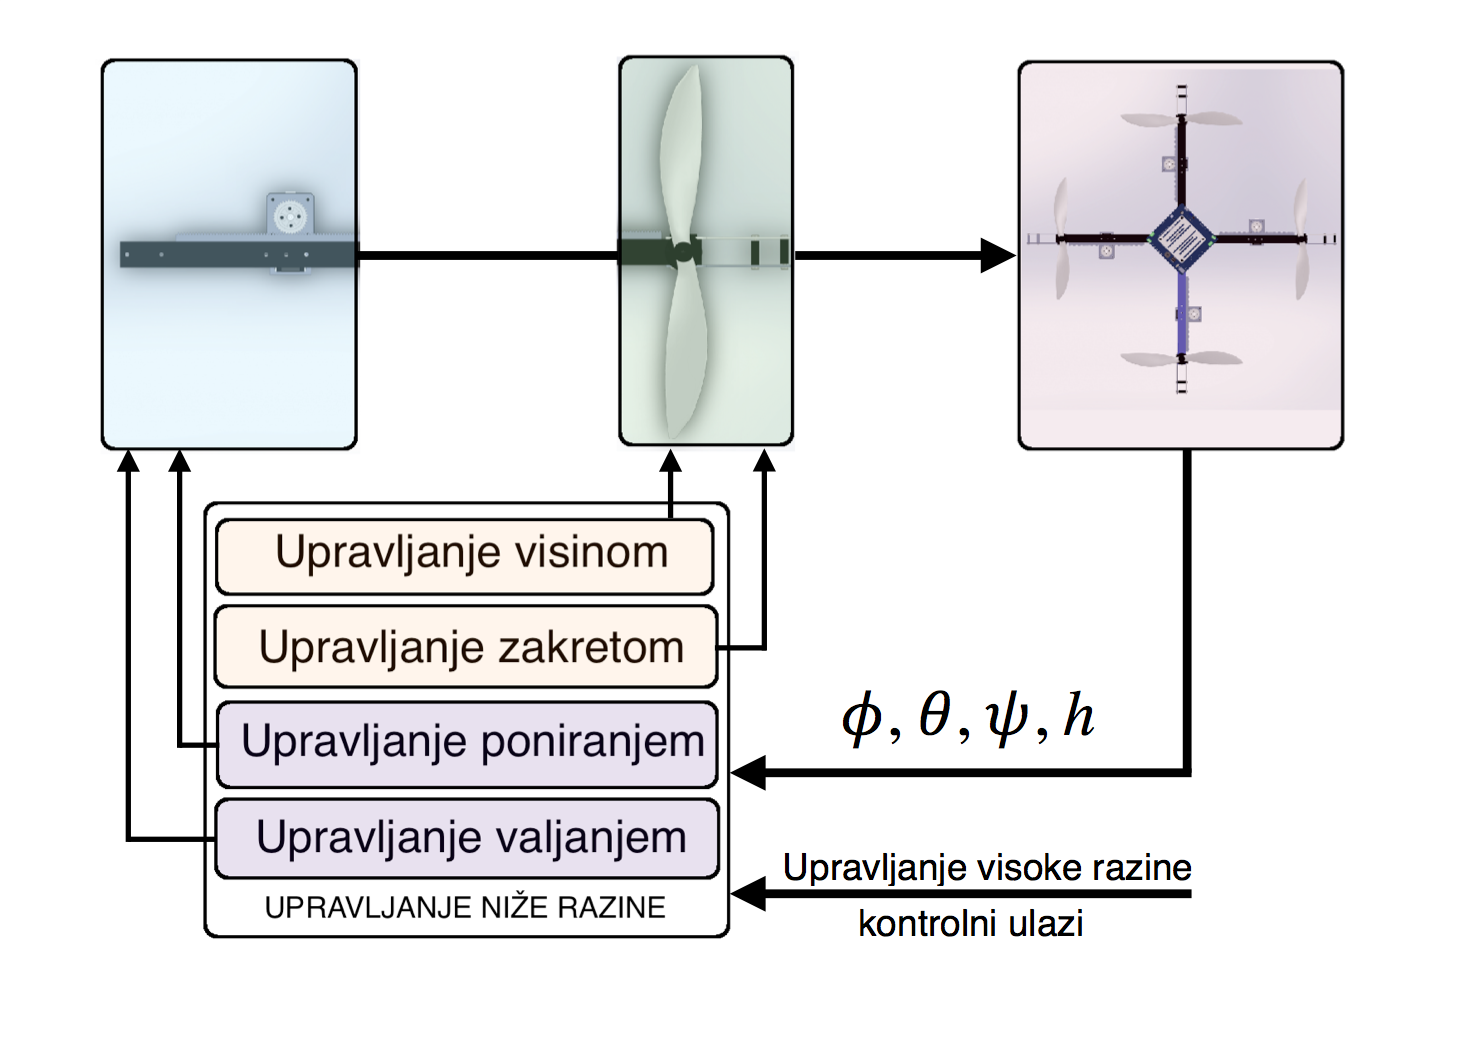
\includegraphics[width=\textwidth]{upr}
	\caption{Upravljačka struktura sustava letjelice}
	\label{fig:upr}
\end{figure}

\newpage

Modeliran je koncept i odabrana je upravljačka struktura, stoga još preostaje odabrati vrstu regulatora te proračunati njegove parametre. Odabire se \textit{P} regulator za upravljanje i unutarnjom i vanjskom petljom. Parametre regulatora, pojačanja $K_{p}$, određujemo koristeći metodu \textit{krivulje mjesta korijena}. Postupak \textit{krivulje mjesta korijena}, ili skraćeno \textit{KMK}, omogućava donošenje zaključka o vladanju zatvorenog regulacijskog kruga na temelju položaja polova i nula prijenosne funkcije otvorenog regulacijskog kruga u kompleksnoj \textit{s} ravnini. Na temelju izgleda KMK-a zaključuje se o stabilnosti zatvorenog regulacijskog kruga \cite{mato}. 

\medskip

Određivanje parametara regulatora obavlja se u dva koraka. Prvo se određuje pojačanje unutarnje petlje prema izrazu za prijenosnu funkciju otvorenog kruga sustava (\ref{eq:tf}) koristeći postupak \textit{krivulje mjesta korijena}. Zatim se određuje prijenosna funkcija zatvorenog kruga unutarnje petlje s prijenosnom funkcijom P regulatora ($K_{p}$) te s prijenosnom funkcijom procesa. Prijenosna funkcija zatvorenog  kruga unutarnje petlje jednaka je prijednosnoj funkciji otvorenog kruga vanjske petlje. Za tu se prijenosnu funkciju postupak ponavlja.  

\medskip

Za određivanje \textit{krivulje mjesta korijena} unutarnje petlje koristi se prijenosna funkcija otvorenog kruga (\ref{eq:tf}) te parametri iz Tablice (\ref{params}). Sustav je stabilan za sva pojačanja za koja se nule i polovi nalaze unutar jedinične kružnice.  Rezultirajući KMK prikazan je Slikom (\ref{fig:unutarnja_Kp}), na kojoj je također prikazan način odabira parametra P regulatora unutarnje petlje. Na slici su prikazana dva očitanja pojačanja. Jedan se nalazi na rubu stabilnosti i jednak je $K= 0.7$. S obzirom na da je to pojačanje na rubu stabilnosti znači da ako se odabere $K_{p} > K$, sustav će postati nestabilan. Iz tog razloga odabire se pojačanje koje polove povlači unutar jedinične kružnice, prikazano drugim očitanjem. Konačan iznos pojačanja P regulatora unutarnje upravljačke petlje jednak je:

 \begin{equation}
 \boxed{
 K_{p,in} = 0.111
 } \ .
 \label{eq:Kp_in}
 \end{equation}


\begin{figure}[H]
	\centering
	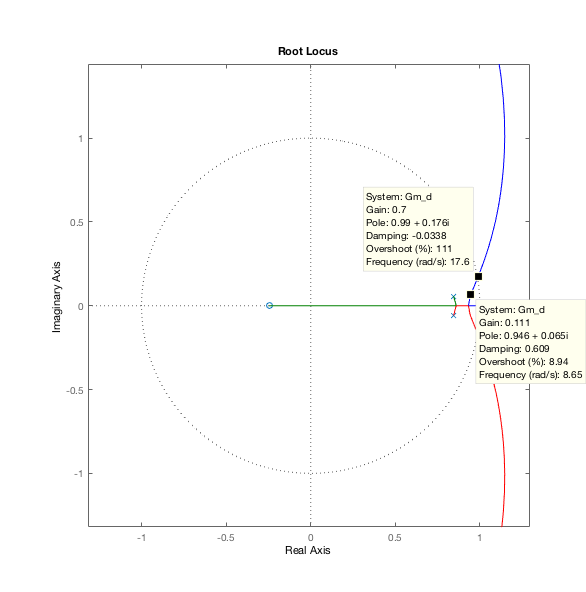
\includegraphics[scale=0.55]{unutarnja_Kp}
	\caption{Odabir pojačanja P regulatora unutarnje upravljačke petlje}
	\label{fig:unutarnja_Kp}
\end{figure}

Stabilnost zatvorenog kruga unutarnje petlje može se ispitati odzivom prijenosne funkcije tog zatvorenog kruga na jediničnu odskočnu pobudu (step) te je taj odziv prikazan Slikom (\ref{fig:step1}):

\begin{figure}[H]
	\centering
	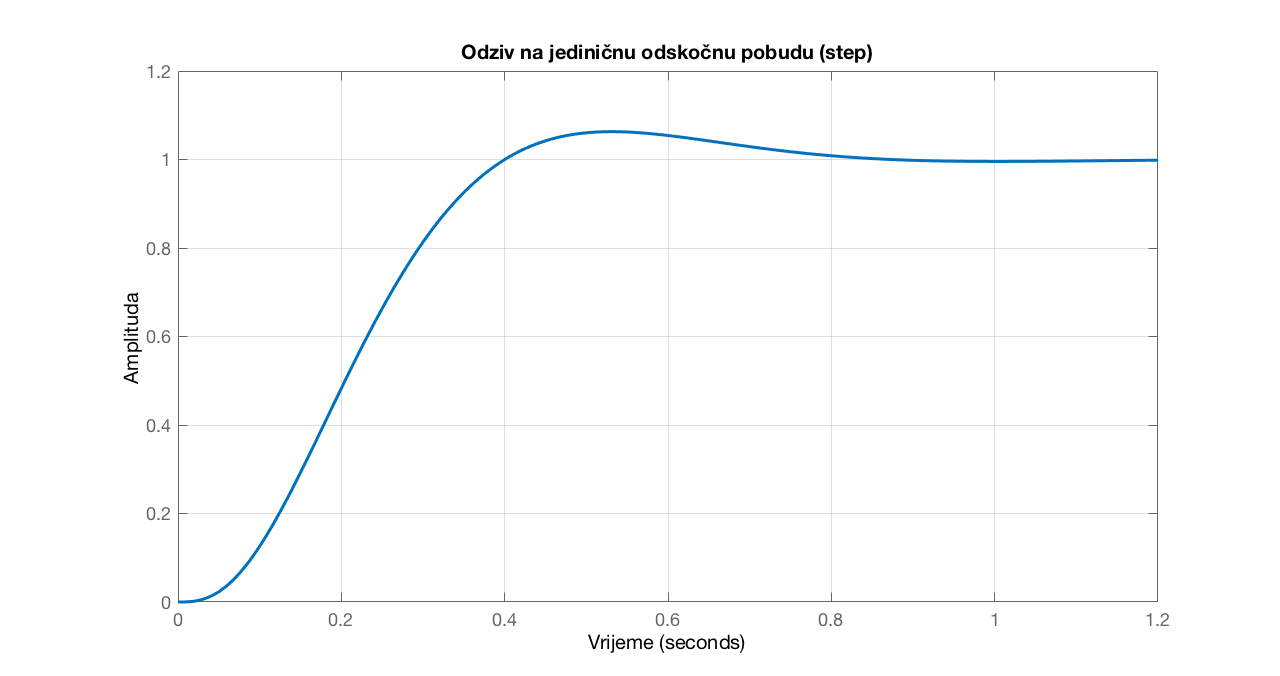
\includegraphics[width=\textwidth]{unutarnja_step}
	\caption{Odziv zatvorenog kruga unutarnje upravljačke petlje na jediničnu odskočnu pobudu}
	\label{fig:step1}
\end{figure}


Analogan postupak primjenjuje se i za vanjsku upravljačku petlju. Prijenosna funkcija otvorenog kruga vanjske petlje jednaka je prijenosnoj funkciji zatvorenog kruga unutarnje petlje:

\begin{equation}
G_{o,out} = \frac{K_{p,in}G_{o,in}}{1 + K_{p,in}G_{o,in}} \ ,
\label{eq:tf2}
\end{equation}

gdje je $K_{p,in} = 0.111$, a $G_{o,in}$  je jednak (\ref{eq:tf}) s uvrštenim parametrima:


\begin{equation}
G_{o,in} = \frac{1}{s(6.4875\cdot10^{-5}s^{2} + 0.0022s  + 0.0210)} \ ,
\label{eq:Goin}
\end{equation}

pa slijedi konačan izraz za $G_{o,out}$:

\begin{equation}
G_{o,out} = \frac{0.111}{6.4875\cdot10^{-5}s^{3} + 0.0022s^{2}  + 0.0210s + 0.111} \ .
\label{eq:Ginz}
\end{equation}
\medskip
\textit{Krivulja mjesta korijena} otvorenog kruga vanjske petlje kao i odabir pojačanja P regulatora prikazano je Slikom (\ref{fig:vanjska_Kp}):

\begin{figure}[H]
	\centering
	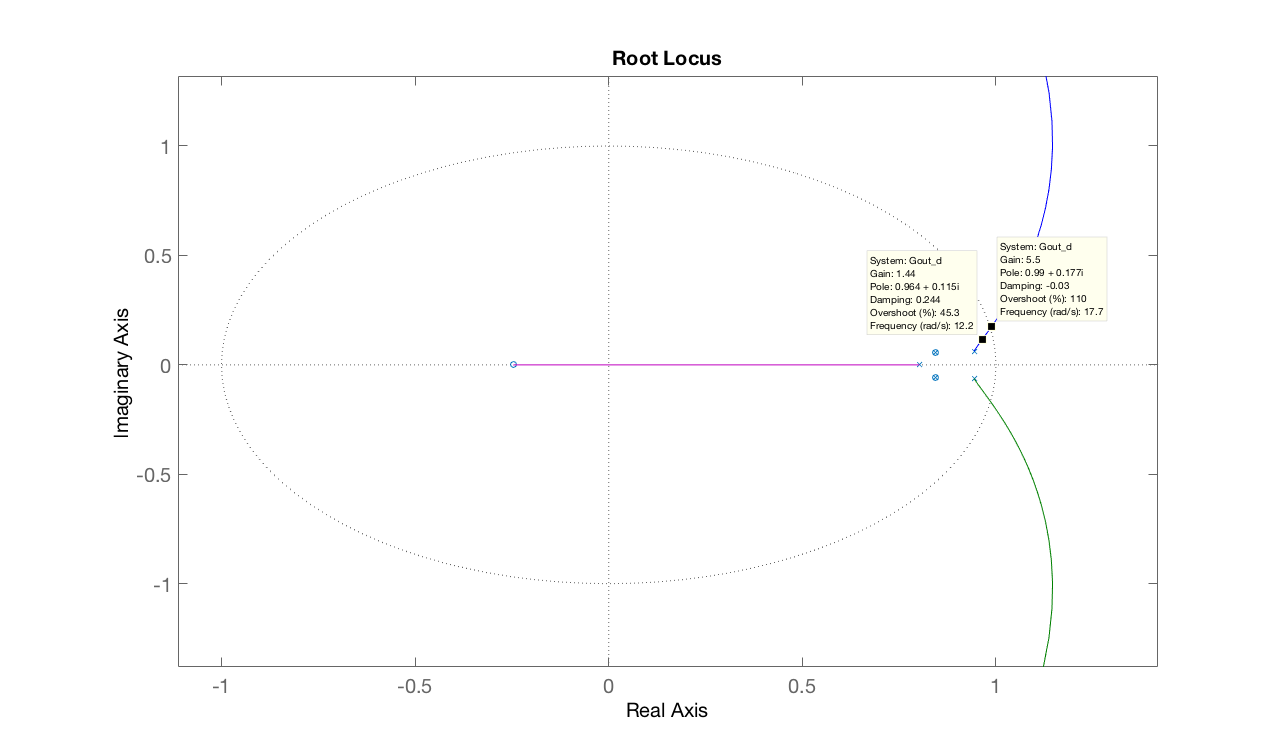
\includegraphics[width=\textwidth]{vanjska_Kp}
	\caption{Odabir pojačanja P regulatora vanjske upravljačke petlje}
	\label{fig:vanjska_Kp}
\end{figure}

\newpage
Konačan iznos pojačanja P regulatora vanjske upravljačke petlje jednak je:
 \begin{equation}
 \boxed{
 K_{p,out} = 1.3
 } \ .
 \label{eq:Kp_out}
 \end{equation}
 
Slijedi opći zapis prijenosne funkcije zatvorenog kruga upravljanja:

\begin{equation}
G_{z,out} = \frac{K_{p,out}G_{o,out}}{1 + K_{p,out}G_{o,out}} \ .
\label{eq:Goutz}
\end{equation}
 
 Konačna prijenosna funkcija zatvorenog kruga upravljanja jednaka je:
 
 \begin{equation}
 G_{o,z} = \frac{0.1443}{6.4875\cdot10^{-5}s^{3} + 0.0022s^{2}  + 0.0210s + 0.2553} \ .
 \label{eq:Goz}
 \end{equation}

Stabilnost zatvorenog kruga vanjske petlje dokazuje se odzivom prijenosne funkcije zatvorenog kruga (\ref{eq:Goz}) na jediničnu odskočnu pobudu (step) te je taj odziv prikazan Slikom (\ref{fig:step2}):

\begin{figure}[H]
	\centering
	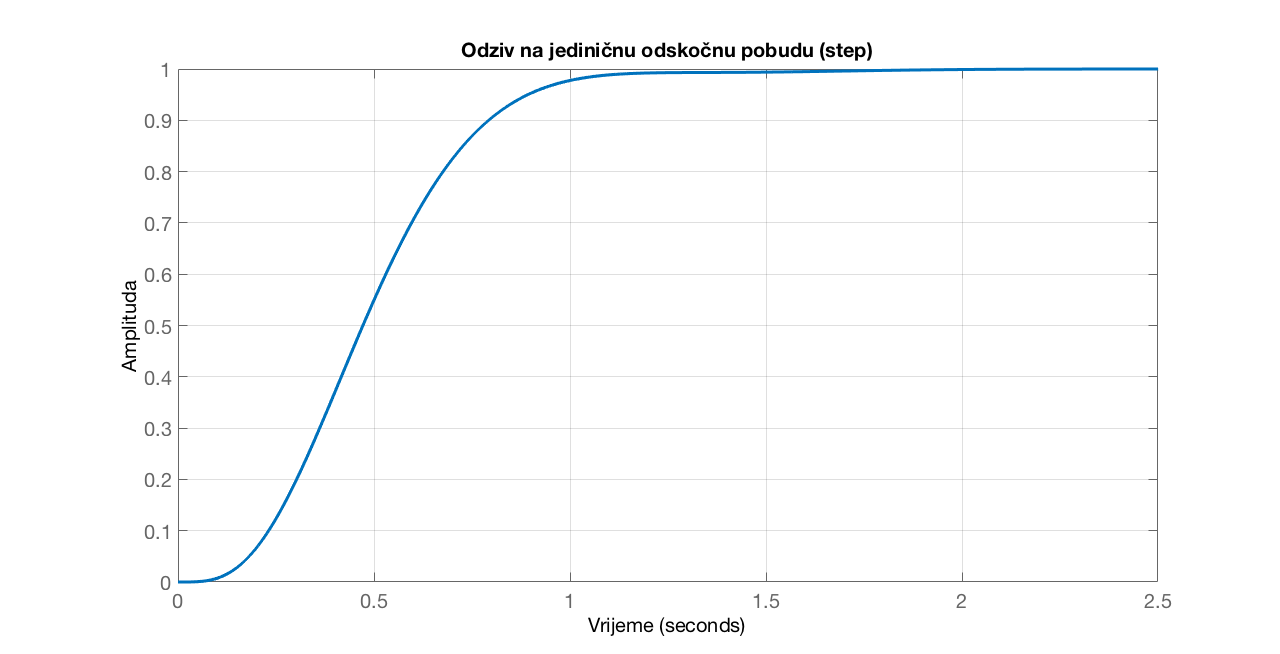
\includegraphics[width=\textwidth]{vanjska_step}
	\caption{Odziv zatvorenog kruga vanjske upravljačke petlje na jediničnu odskočnu pobudu}
	\label{fig:step2}
\end{figure}


\end{document}